\documentclass[12pt,a4paper]{report}
\usepackage[left=2.5cm,right=2.5cm,top=3cm,bottom=3cm]{geometry}
\usepackage{fancyhdr}
\usepackage{etoolbox}
\usepackage{titlesec}
\usepackage{titling} % para personalizar el título
\usepackage{amssymb}
\usepackage{amsmath}
\usepackage{graphicx}
\usepackage{ulem}
\usepackage{cancel}
\usepackage{enumitem}
\usepackage{lmodern}
\usepackage{tikz}

\allowdisplaybreaks

\pagestyle{fancy}
\fancyhf{} 
\fancyhead[L]{UTN-FRC}
\fancyhead[C]{ASyS}
\fancyhead[R]{2R3}
\renewcommand{\headrulewidth}{0.4pt}
\fancyfoot[C]{\vfill\thepage}

\patchcmd{\chapter}{\thispagestyle{plain}}{\thispagestyle{fancy}}{}{}

\renewcommand{\chaptername}{Ejercicio}

\usetikzlibrary{calc, arrows.meta, positioning}

\titleformat{\chapter}[display]
  {\normalfont\bfseries}{\chaptertitlename\ \thechapter}{15pt}{}
\titlespacing*{\chapter}{0pt}{-30pt}{-30pt}

\setlength{\headheight}{15pt}

\DeclareMathSizes{17}{15}{10}{10}

\setlength{\parskip}{6pt}

\title{%
  \fontsize{25}{0}\selectfont Universidad Tecnológica Nacional \\
  \fontsize{22}{30}\selectfont Analisis de Señales y Sistemas \\
  \fontsize{20}{25}\selectfont Trabajo Practico 2
}
\author{
Alejo Agustin Lopez Demichelis\\
Franco Palombo\\
Ignacio Gil\\
Jesus Agustin Frigerio\\
Laureano Valentin Reinoso\\
Luciano Tomas Cortesini Perez\\
Matias Gabriel Moran\\
Leonardo Ramos\\
}
\date{19 / 08 / 2024}

\begin{document}
\maketitle

\chapter{}%ejercicio 1

\textbf{Movimiento Rectilíneo Uniformemente Variado (MRUV) - Caída libre}

\begin{itemize}[left=0pt]
  \item Un primer cuerpo de masa $m_1$ se deja caer (verticalmente) desde una posición inicial $y_0 > 0$.

  \item Un segundo cuerpo de igual masa que el primero, se deja caer (verticalmente) desde una posición inicial 
     $\frac{1}{2} y_0$, es decir, a mitad de camino del primer cuerpo.

\end{itemize}

Teniendo como punto de referencia el "suelo", responder las siguientes consignas:

\begin{enumerate}[label=\alph*),left=0pt]
  \item Realizar un gráfico que represente la situación de los dos cuerpos en caída libre, sus respectivos vectores 
    de velocidad y posición.

  \item Determinar las ecuaciones de cinemáticas para la posición $y_1(t)$ y $y_2(t)$ en función del tiempo para cada
    uno de los cuerpos, respectivamente. \textbf{Reflexionar:} ¿las funciones $y_1, y_2$ pueden interpretarse como 
    señales de variable de tiempo continuo? ¿Las masas de los cuerpos intervienen en la descripción de las funciones
    $y_1(t),y_2(t)$?

    Partimos primero de la ecuacion que determina la posicion de un cuerpo con aceleracion uniforme:
    $$Y(t) = Y_0 + V_0 t + \frac{1}{2} g t^2$$
    Para ambos casos asumimos la velocidad inicial $V_0 = 0$, despreciamos la resistencia del aire y tomamos como valor de aceleracion de la gravedad $g = 9.8 \frac{m}{s^2}$:
    $$y_1(t) = Y_0 - \frac{1}{2}9,8\frac{m}{s^2}t^2$$
    $$y_2(t) = \frac{Y_0}{2} - \frac{1}{2}9,8\frac{m}{s^2}t^2$$

    Como se puede observar, las masas no aparecen en las ecuaciones de $y_1(t)$ y $y_2(t)$, por lo que se deduce que las masas no intervienen en la descripcion de las funciones.

  \item Calcular el tiempo de vuelo (total) $T$ del primer cuerpo, en función de $y_0$. Similarmente, calcular el
    tiempo de vuelo $\tau$ del segundo cuerpo. ¿Qué relación aritmética encuentra entre los dos tiempos $T$ y $\tau$?
    ¿Se puede obtener $y_2$ como un escalonado en el tiempo de la señal $y_1$?

    Se obtienen los tiempos $T$ y $\tau$ como:
    $$T = \sqrt{\frac{2h}{g}}$$
    $$\tau = \sqrt{\frac{h}{g}}$$
    La relacion aritmetica entonces:
    $$\frac{T}{\tau} = \frac{\sqrt{2}\sqrt{gh}}{\sqrt{gh}}$$
    $$T = \sqrt{2}\tau$$

    No se puede obtener $y_2(t)$ como un escalonado de tiempo de $y_1(t)$. Al escalar el tiempo de $y_1(t)$ por un factor de $\sqrt{2}$ queda $y_1(t) = Y_0 - \frac{1}{2}g(\sqrt{2}t)^2$. T y $\tau$ coinciden, es decir los tiempo finales son iguales, pero no coinciden las funciones de posicion. Es importante notar que, aunque existe esta relacion entre los tiempos de vuelo, no es fisicamente correcto interpretar la posicion $y_2(t)$ del segundo cuerpo como una version escalada temporalmente de $y_1(t)$. Los dos cuerpos tienen trayectorias y tiempos de vuelo diferentes debido a sus diferentes alturas iniciales, y cada uno debe ser tratado de manera independiente.


  \item Calcular el tiempo $t_0$ que le toma al primer cuerpo estar en la posición $\frac{1}{2} y_0$. ¿Qué relación 
    aritmética encuentra entre $t_0$ y $\tau$? ¿Se puede obtener $y_2$ como una traslación temporal de la señal $y_1$?

    $$\frac{y_0}{2} = Y_0 - \frac{1}{2}g{t_0}^2$$
    $$(\frac{y_0}{2} - Y_0) \cdot (\frac{-2}{g}) = {t_0}^2$$
    $$-\frac{y_0}{2} \cdot (\frac{-2}{g}) = {t_0}^2$$
    $$\sqrt{\frac{y_0}{g}} = t_0$$
    $$t_0 = t$$

    No se puede obtener $y_2(t)$ como una traslacion temporal de $y_1(t)$, porque al desplazar temporalmente $y_1(t)$, este no coincide con $y_2(t)$, sin embargo para el $t_0 = t$ si coinciden las posiciones.

  \item \textbf{Reflexionar:} ¿Tiene sentido físico evaluar la señal $y_1$ en tiempos $t > T$? Similarmente, ¿tiene 
    sentido físico evaluar la señal $y_2$ en tiempos $t > \tau$? En caso afirmativo, ¿cuál es la interpretación
    física? Y en caso negativo, emplear alguna herramienta para redefinir las señales $y_1, y_2$, de tal forma que la 
    información provista por el futuro sea nula. Por otra parte, ¿tiene sentido físico evaluar a las señales $y_1,
    y_2$ en tiempos negativos $t < 0$? En caso afirmativo, ¿qué representa? Y en caso negativo, emplear alguna 
    herramienta para redefinir las señales $y_1, y_2$ de tal forma que la información provista por el pasado sea nula.

    No tiene sentido físico evaluar las señales $y_1(t)$ ni $y_2(t)$ en tiempos mayores a T y $\tau$ respectivamente. A su vez tampoco tiene sentido evaluar las señales en tiempos negativos, menores a cero. Podríamos definir las señales como:
    $$y_1(t) = (Y_0 + V_0t - \frac{1}{2}gt^2)u(t)u(T - t)$$
    $$y_2(t) = (\frac{Y_0}{2} + V_0t - \frac{1}{2}gt^2)u(t)u(\tau - t)$$

  \item Teniendo en cuenta las señales redefinidas del inciso anterior $y_1, y_2$ (pasado y futuro de la señal son
    nulos) verificar si estas cumplen (o no) cada una de las siguientes propiedades: Periódica, Energía finita,
    Potencia finita, causal, acotada.

\begin{enumerate}[label=\alph*)]
    \item Periodicidad

    Las señales $y_1(t)$ y $y_2(t)$ no son periódicas, ya que representan la posición de los cuerpos en caída libre y no se repiten en intervalos regulares de tiempo. Cada cuerpo cae una vez y llega al suelo, después de lo cual la señal es nula.
    \item Energia

    Las señales $y_1(t)$ e $y_2(t)$ tienen una duración finita en el tiempo (desde t = 0 hasta t = T para $y_1(t)$ y hasta t = $\tau$ para $y_2(t)$), y son nulas fuera de estos intervalos, por lo tanto su energía es finita.
    \item Potencia

    Dado que las señales $y_1(t)$ e $y_2(t)$ tienen energía finita, se puede afirmar que tienen una potencia media igual a cero.
    \item Causaludad

    Ambas señales son causales por el hecho de estar multiplicadas por los escalones unitarios (u(t)u(T - t) para $y_1(t)$ y  u(t)u($\tau$ - t) para $y_2(t)$) que anulan el pasado y futuro de las mismas.
    \item Modulo

    Las señales $y_1(t)$ e $y_2(t)$ son acotadas en sus respectivos intervalos de tiempo. Para $y_1(t)$ la máxima magnitud ocurre en t = 0 y es $Y_0$. Para $y_2(t)$ la máxima magnitud también ocurre en t = 0  y es $\frac{1}{2}Y_0$.
\end{enumerate}

\end{enumerate}

\textbf{Movimiento Armónico Simple (MAS) - Masa/Resorte}

Considerar un sistema conformado por una Masa $m$, atada a la derecha de un resorte con constante elástica $\kappa$, 
dispuesto en forma horizontal y sujetado en el extremo izquierdo. Teniendo como punto de referencia la posición de
equilibrio, máxima amplitud $A > 0$ y despreciando los efectos de la fricción, responde las siguientes consignas:

\begin{enumerate}[label=\alph*),left=0pt]
  \item Realizar un gráfico que represente el sistema y sus respectivos vectores de fuerza.

  \item Determinar la ecuación de cinemática para la posición $x(t)$ en función del tiempo. \textbf{Reflexionar:} ¿la
    función $x$ puede interpretarse como una señal de variable de tiempo continua?

    Partiendo de la ecuacion diferencial de un oscilador armonico simple $m \frac{dt^2}{d^2x} + kx = 0$, determinamos la ecuacion de cinematica para la posicion en funcion del tiempo $x(t) = A \sin(\omega t + \phi)$. Si, la funcion $x(t)$ puede interpretarse como una señal de variable de tiempo continuo.

  \item Es de conocimiento general que la función posición $x(t)$ se puede determinar en función del $seno$ o del
    coseno. Determinar la transformación temporal sobre la señal, la cual permite pasar de la formulación $seno$ a la
    formulación $coseno$.

    Para pasar de la formulación seno a la formulación coseno debe aplicarse una traslación temporal a la señal correspondiente al desfase entre las funciones trigonométricas seno y coseno, es decir sumar $\frac{\pi}{2}$. Entonces:

    $$A \sin(\omega t + \frac{\pi}{2}) = A \cos(\omega t)$$

  \item Verificar si la señal $x(t)$ cumple (o no) cada una de las siguientes propiedades: Periódica, Energía finita,
    Potencia finita, causal, acotada.

  \begin{enumerate}[label=\alph*)]
    \item Periodica

      Es periodica ya que existe un valor T tal que $x(t) = x (t + nT)$, donde n = 1,2,3..
    \item Energia

    Tiene energia infinita. Para señales periodicas, la energia total en el sentido clasico puede ser infinita debido a que la señal se repite indefinidamente, pero si hablamos de la energia en un periodo T, es finita y es:

    $$E_T = \int_{0}^{T} |A \cos(\omega t)|^2 dt$$
    $$E_T = A^2 \int_{0}^{T} \cos(\omega t)^2 dt$$
    $$E_T = A^2 \int_{0}^{T} \frac{1 + \cos(2 \omega t)}{2} dt$$
    $$E_T = A^2 \frac{1}{2}\int_{0}^{T}  \cos(2 \omega t)dt$$
    \item Potencia

    Tiene energia infinita si consideramos el intervalo $(-\infty,\infty$, pero la energia es finita en un solo periodo, por lo que la potencia media es finita:

    $$P_{med} = \lim_{T \to \infty} \frac{1}{2T} E_T$$
    $$P_{med} = \lim_{T \to \infty} \frac{A^2T}{4T} = \frac{A^2}{4}$$
    $$P_T = 2 P_{med} = \frac{A^2}{2}$$
    \item Acotada

    La señal es acotada ya que para todo t, $x(t) <= A$ siendo A la amplitud. Esto se da ya que las funciones trigonometricas seno o coseno toman valores entre -1 y 1
    \item Causal

    La señal no es causal porque esta definida para todos los tiempos, $t \in (-\infty,\infty)$
  \end{enumerate}
\end{enumerate}

\chapter{}%ejercicio 2
Considerar las siguientes señales proporcionadas por un rectificador de onda completa y $1/2$ onda respectivamente:
\textbf{Señal Sinusoidal rectificada de onda completa}, $x_1(t)$ determinada por el gráfico:

% Incluir aquí el gráfico de la señal sinusoidal rectificada de onda completa

\textbf{Señal Sinusoidal rectificada de media onda}, $x_2(t)$ determinada por el gráfico:

% Incluir aquí el gráfico de la señal sinusoidal rectificada de media onda

\begin{enumerate}[label=\alph*),left=0pt]
  \item Calcular el periodo fundamental $T_0$ de las señales $x_1, x_2$. ¿Las señales tienen energía finita? Calcular
    la energía relativa a un intervalo con longitud un periodo fundamental $T_0$.

  \item Teniendo en cuenta que la potencia media de una señal se define como

  $$P_1 = \lim_{r \to \infty} \frac{1}{2r} \int_{-r}^{r} |x(t)|^2 \, dt$$

    \begin{itemize}[left=0pt]
    \item Demostrar la siguiente igualdad, válida para señales periódicas en donde la potencia media relativa a un
      intervalo con longitud un periodo fundamental $T_0$ coincide con la potencia media, es decir:

     $$P_1 = \frac{1}{T_0} \int_{t_0}^{t_0 + T_0} |x(t)|^2 \, dt$$

    \item Calcular la potencia media $P_1$ de la señal $x_1$ y similarmente, $P_2$ de la señal $x_2$.

  \end{itemize}

  \item Considerar el conjunto de señales básicas

  $$\{\psi_n(t) = \cos(n\omega t) \mid n \geq 0\} \cup \{\varphi_n(t) = \sin(n\omega t) \mid n \geq 1\}$$

    \begin{itemize}[left=0pt]
    \item Calcular la energía relativa a un intervalo con longitud un periodo fundamental $T_0$ y el periodo $T_n$
      de cada señal del conjunto, y luego, demostrar que (dos a dos) forman un conjunto de señales ortogonales más no
      ortonormales.

      \textbf{Reflexión:} ¿si los periodos $T_n$ de cada señal del conjunto básico son distintos, por qué la suma 
      (finita/infinita) es periódica? ¿Por qué se restringe el dominio del tiempo en un intervalo del tipo 
      $t_0 \leq t \leq t_0 + T_0$, si las señales básicas están bien definidas en todo el eje temporal?

   \item Obtener la representación de las señales $x_1, x_2$ como una combinación lineal de las señales básicas, 
     esto es, calcular coeficientes $(a_n, b_n)$ en $\mathbb{R}$ tales que:

     $$x_1 = \sum_{n=0}^{\infty} a_n \psi_n + \sum_{n=1}^{\infty} b_n \varphi_n$$
     Similarmente para la señal $x_2$.

   \item Truncar la suma infinita del inciso anterior en $n = 5$ y hacer un gráfico comparativo entre la señal 
     original $x_1$ y su aproximación trigonométrica. Similarmente para la señal $x_2$.

  \end{itemize}

  \item Considerar el conjunto de señales básicas

  $$\{\phi_n(t) = e^{jn\omega t} \mid n \in \mathbb{Z}\}$$

  Notar que la siguiente relación entre las señales con parámetro negativo y el conjugado:

  $$\phi(-n) = \phi_n^*, \forall n \geq 0$$

  \begin{itemize}[left=0pt]

    \item Calcular la energía relativa a un intervalo con longitud un periodo fundamental $T_0$ y el periodo $T_n$ de
      cada señal del conjunto, y luego, demostrar que (dos a dos) forman un conjunto de señales ortogonales más no
      ortonormales.\newline
      \textbf{Reflexión:} ¿si los periodos $T_n$ de cada señal del conjunto básico son distintos, por qué la suma
      (finita/infinita) es periódica? ¿Por qué se restringe el dominio del tiempo en un intervalo del tipo 
      $t_0 \leq t \leq t_0 + T_0$, si las señales básicas están bien definidas en todo el eje temporal?

    \item Obtener la representación de las señales $x_1, x_2$ como una combinación lineal de las señales básicas, esto 
      es, obtener coeficientes $C_n$ en $\mathbb{C}$ tales que

      $$x_1 = \sum_{-\infty < n < \infty} C_n \phi_n =
      \sum_{n=1}^{\infty} C_{-n} \phi_n^* + C_0 \phi_0 + \sum_{n=1}^{\infty} C_n \phi_n$$

      Similarmente para la señal $x_2$.

    \item Considerar $|n| \leq 5$ y realizar el espectro de frecuencias de ambas señales en fase, esto es, graficar los 
      pares ordenados

      $$\{(n, \text{Arg}(C_n)) \mid -5 \leq n \leq 5\}$$
      correspondientes a cada señal $x_1, x_2$.

      \item Considerar $|n| \leq 5$ y realizar el espectro de frecuencias de ambas señales en módulo, esto es, graficar 
        los pares ordenados

      $$\{(n, |C_n|) \mid -5 \leq n \leq 5\}$$

      correspondientes a cada señal $x_1, x_2$.\newline

    \item Calcular una aproximación a las potencias medias $P_1, P_2$, por medio de la relación de Parseval con los 
      espectros de frecuencia de ambas señales en módulo (usar la información de los incisos anteriores) y discriminar 
      el aporte de las componentes (CC, AC).

      \textbf{Reflexionar:} ¿Qué ventajas/desventajas encuentra entre el método directo para calcular la potencia media 
      $P_1, P_2$ de las señales $x_1, x_2$ en la variable de tiempo $t$ y el método que se deriva de la relación de 
      Parseval, en donde los cálculos se realizan en la variable $n \in \mathbb{Z}$?

  \end{itemize}

  \item Comparar los espectros obtenidos para cada una de las señales $x_1, x_2$, evaluar y proponer las 
    características sobresalientes de ambos espectros.
\end{enumerate}

\chapter{}%ejercicio 3

Considerar $G_T(t) = \mu_{(t + \frac{T}{2})} - \mu_{(t - \frac{T}{2})}$ una señal pulso rectangular con duración finita
$T$ y amplitud unitaria.

\begin{enumerate}[label=\alph*),left=0pt]

  \item Realizar el gráfico de las señales $x_1 = G_1(t)$ y $x_2 = G_{0.1}(t)$, luego, calcular la energía $E_1$ de 
    $x_1$, y similarmente $E_2$ de $x_2$.

    \begin{figure}[h!]
      \hspace{6mm}
      \begin{minipage}{0.45\textwidth}
        \centering
        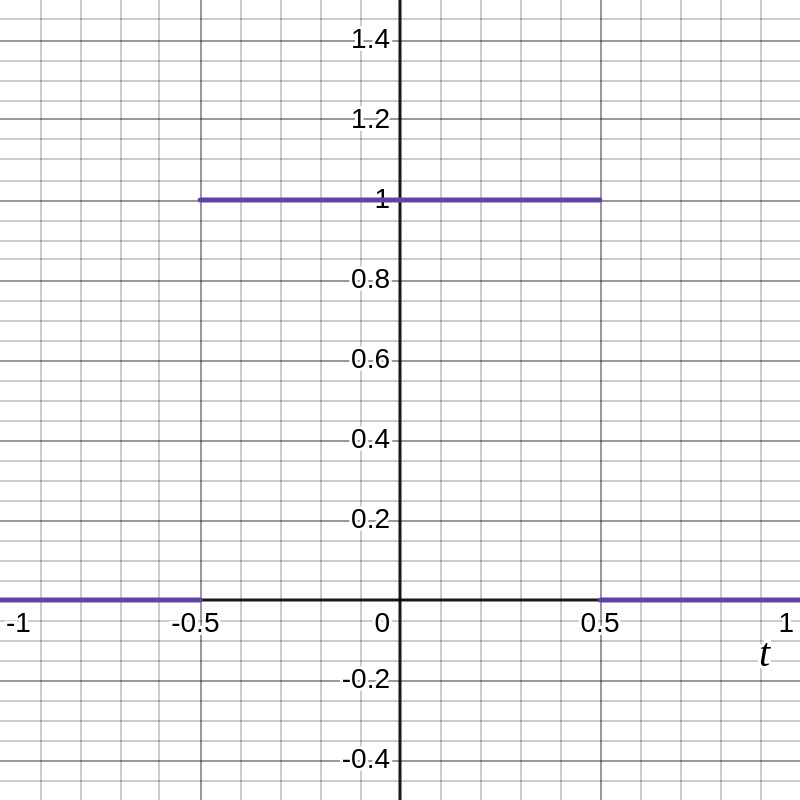
\includegraphics[width=\textwidth]{images/ej3.1}
        \caption{Grafico de la señal $x_1$}
        \label{fig:imagen1}
      \end{minipage}
      \hfill
      \begin{minipage}{0.45\textwidth}
        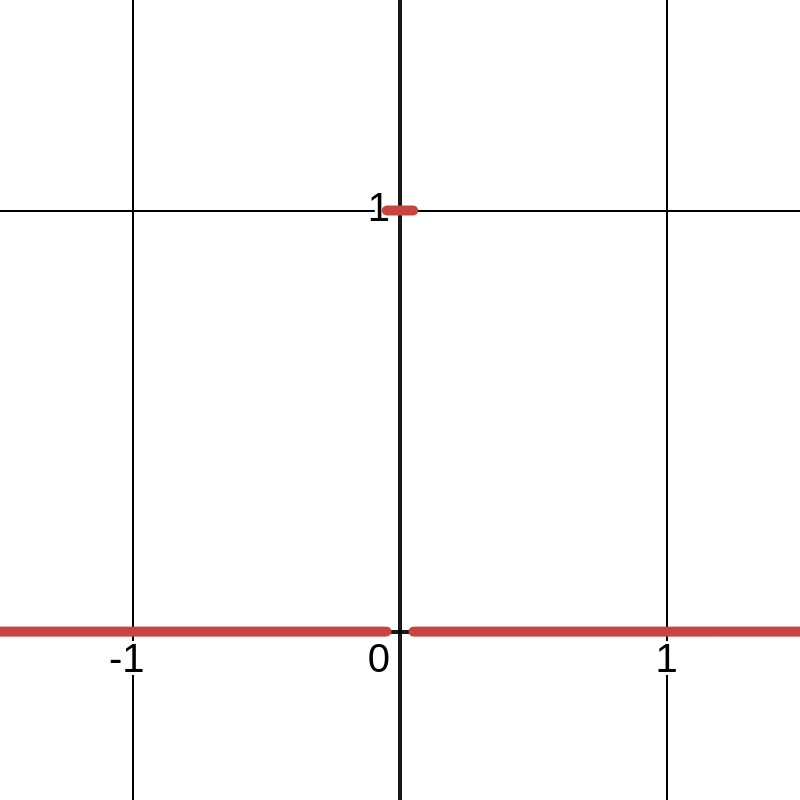
\includegraphics[width=\textwidth]{images/ej3.2}
        \caption{Grafico de la señal $x_2$}
        \label{fig:imagen2}
      \end{minipage}
    \end{figure}

    Para calcular la energia de cada respectiva señal aplicamos la definición:
    $$E_x = \int_{-\infty}^{\infty}x_t^2dt$$
    En este caso, por ser una señal de amplitud 1, simplemente es el area encerrada bajo cada una de las curvas
    $$E_1 = \int_{-\infty}^{\infty}x_1^2dt= \int_{-0,5}^{0,5}1dt=1$$
    $$E_2 = \int_{-\infty}^{\infty}x_2^2dt= \int_{-0,05}^{0,05}1dt=0.1$$

  \item Obtener la transformada de Fourier $F_1(\omega) = \mathcal{F}\{x_1\}$ y similarmente $F_2(\omega) =
    \mathcal{F}\{x_2\}$. Reflexionar: ¿En qué variable están definidas las funciones $F_1, F_2$? 
    ¿Qué representa la variable $\omega$ y qué diferencia tiene con la variable $t$? 
    ¿Las funciones $F_1, F_2$ resultan periódicas?

    La transformada de furier para una un pulso genérico $G_T$ es:

    $$\mathcal{F}\{G_T\} = \int_{-\infty}^{\infty}G_T e^{-jwt}dt$$

    Pero, como $G_T$ es 1 en el intervalo $(-\frac{T}{2},\frac{T}{2})$ y 0 en el resto.

    $$
    \begin{aligned}
      \mathcal{F}\{G_T\} &= \int_{-\frac{T}{2}}^{\frac{T}{2}}e^{-jwt}dt \\[6pt]
      \mathcal{F}\{G_T\} &= -\frac{e^{-jwt}}{jw}\Big|^{\frac{T}{2}}_{-\frac{T}{2}} \\[6pt]
      \mathcal{F}\{G_T\} &= -\frac{e^{\frac{-jwT}{2}}-e^{\frac{jwT}{2}}}{jw}\\[6pt]
      \text{como:} \hspace{2mm} sin(&x)=\frac{e^{jx}-e^{-jx}}{2j}\\[6pt]
      \mathcal{F}\{G_T\} &= \frac{2}{w}sin\Big(\frac{wT}{2}\Big)
    \end{aligned}
    $$

    Por ende para la señal $x_1$ la transformada será:
    $$F_1= \frac{2}{w}sin\Big(\frac{w}{2}\Big)$$

    Y para $x_2$ la transformada será:
    $$F_1= \frac{2}{w}sin\Big(\frac{w}{20}\Big)$$

    \begin {itemize}[left=0pt]

      \item Graficar el espectro de frecuencia en fase para $F_1, F_2$, esto es, graficar los pares ordenados
        $$\{(\omega, \text{Arg}(F)) \mid \omega \in \mathbb{R}\}$$
        Para cada una de las funciones $F_1, F_2$.\newline

        \begin{figure}[h!]
          \hspace{10mm}
          \begin{minipage}{0.45\textwidth}
            \centering
            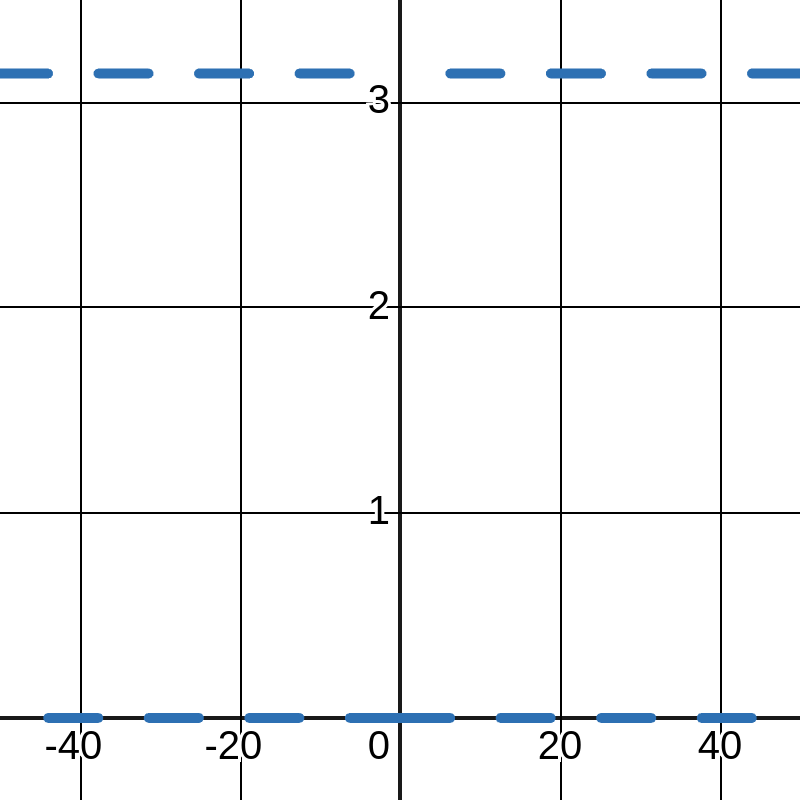
\includegraphics[width=\textwidth]{images/ej3.3}
            \caption{Espectro de frecuencia en fase para $x_1$}
            \label{fig:imagen1}
          \end{minipage}
          \hfill
          \begin{minipage}{0.45\textwidth}
            \centering
            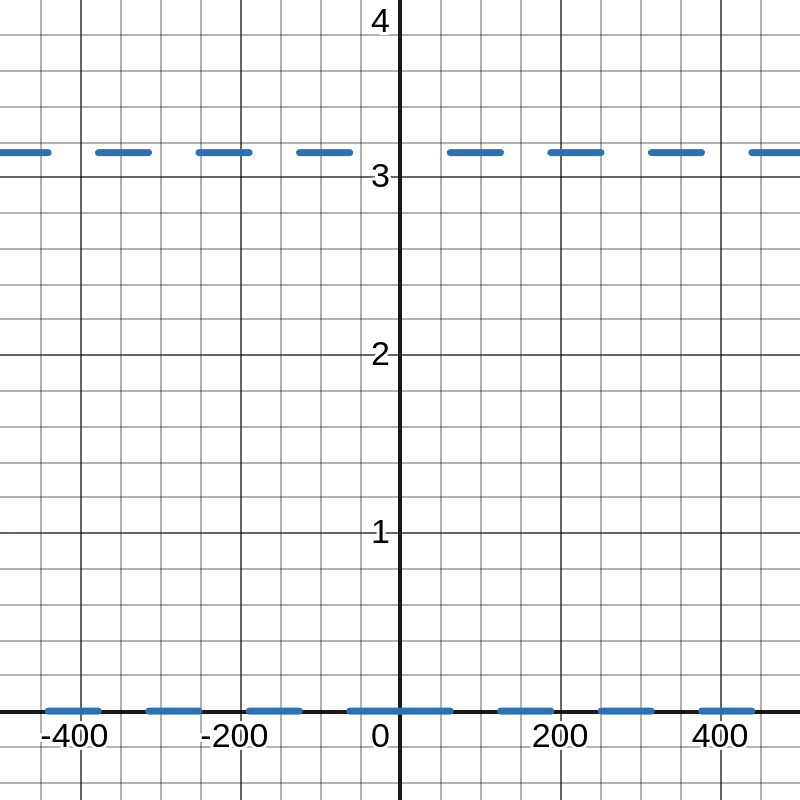
\includegraphics[width=\textwidth]{images/ej3.4}
            \caption{Espectro de frecuencia en fase para $x_2$}
            \label{fig:imagen2}
          \end{minipage}
        \end{figure}

        \textbf{Reflexionar:} ¿El espectro de frecuencia en fase es discreto o continuo? ¿El gráfico admite una simetría
        par, impar o ninguna?\\

        En ambos casos, el espectro de la frecuencia en fase es una señal de tiempo continuo y admite simetria par.\\

      \item Graficar el espectro de frecuencia en módulo para $F_1, F_2$, esto es, graficar los pares ordenados
        $$\{(\omega, |F|) \mid \omega \in \mathbb{R}\}$$
        Para cada una de las funciones $F_1, F_2$.\newline

        \begin{figure}[h!]
          \hspace{10mm}
          \begin{minipage}{0.45\textwidth}
            \centering
            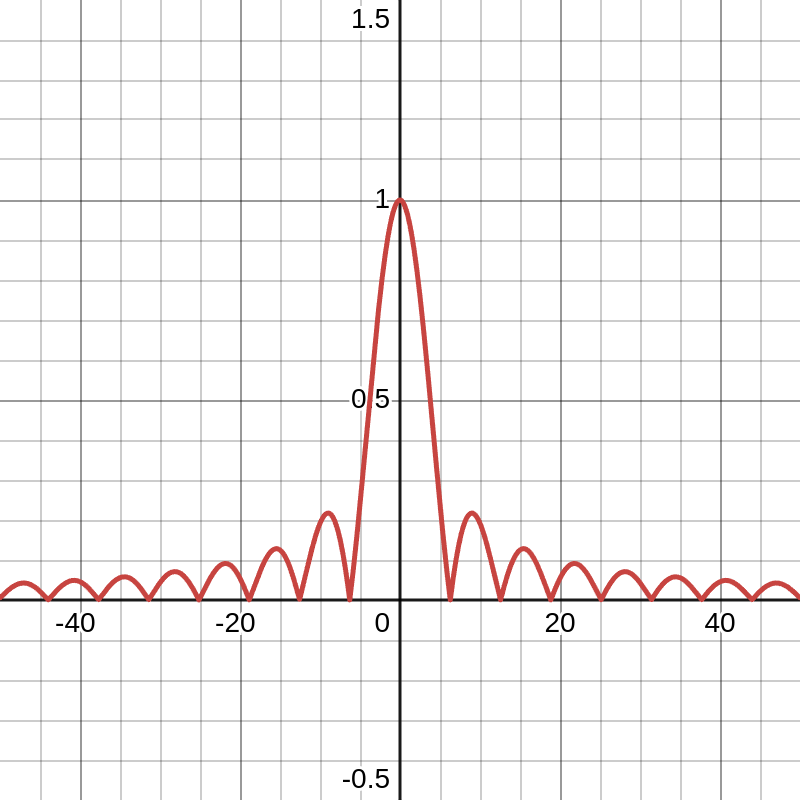
\includegraphics[width=\textwidth]{images/ej3.5}
            \caption{Espectro de frecuencia en módulo para $x_1$}
            \label{fig:imagen1}
          \end{minipage}
          \hfill
          \begin{minipage}{0.45\textwidth}
            \centering
            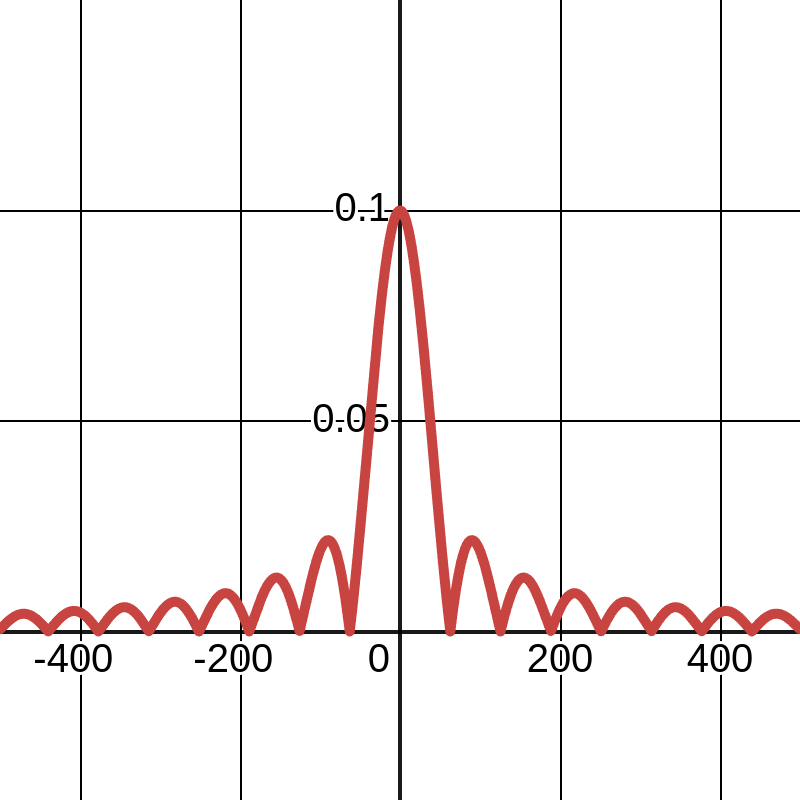
\includegraphics[width=\textwidth]{images/ej3.6}
            \caption{Espectro de frecuencia en módulo para $x_2$}
            \label{fig:imagen2}
          \end{minipage}
        \end{figure}

        \textbf{Reflexionar:} ¿El espectro de frecuencia en módulo es discreto o continuo? ¿El gráfico admite una 
        simetría par, impar o ninguna?\\

        Para ambas señales el espectro de frecuencia en modulo es una señal de tiempo continuo, y admiten simtria par.\\

      \item Graficar la densidad espectral para $F_1, F_2$, esto es, graficar los pares ordenados
        $$\{(\omega, |F|^2) \mid \omega \in \mathbb{R}\}$$
        Para cada una de las funciones $F_1$, $F_2$.\\

        \begin{figure}[h!]
          \hspace{10mm}
          \begin{minipage}{0.45\textwidth}
            \centering
            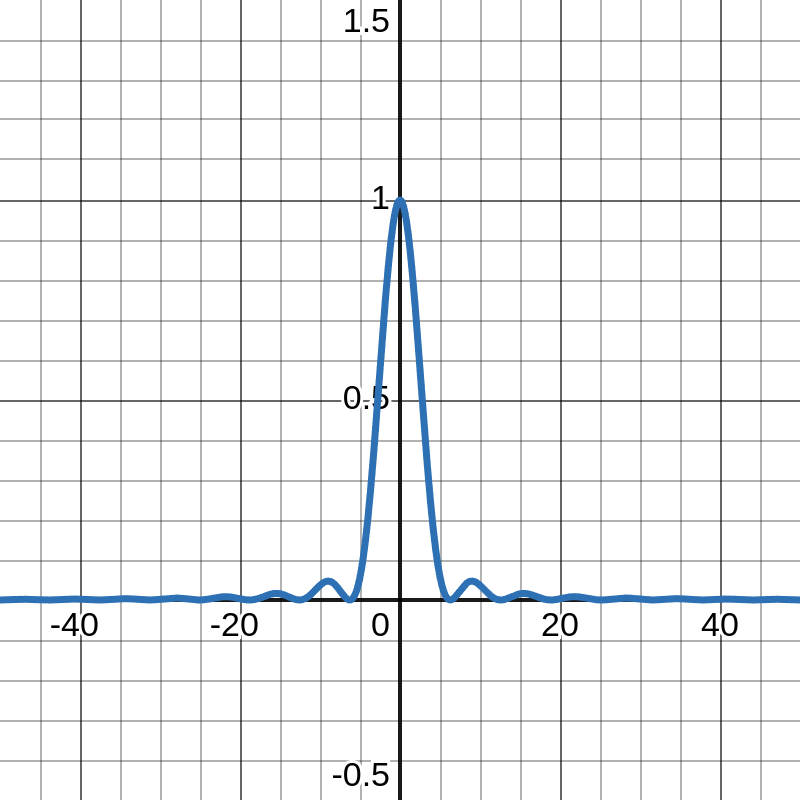
\includegraphics[width=\textwidth]{images/ej3.7}
            \caption{Densidad espectral para $x_1$}
            \label{fig:imagen1}
          \end{minipage}
          \hfill
          \begin{minipage}{0.45\textwidth}
            \centering
            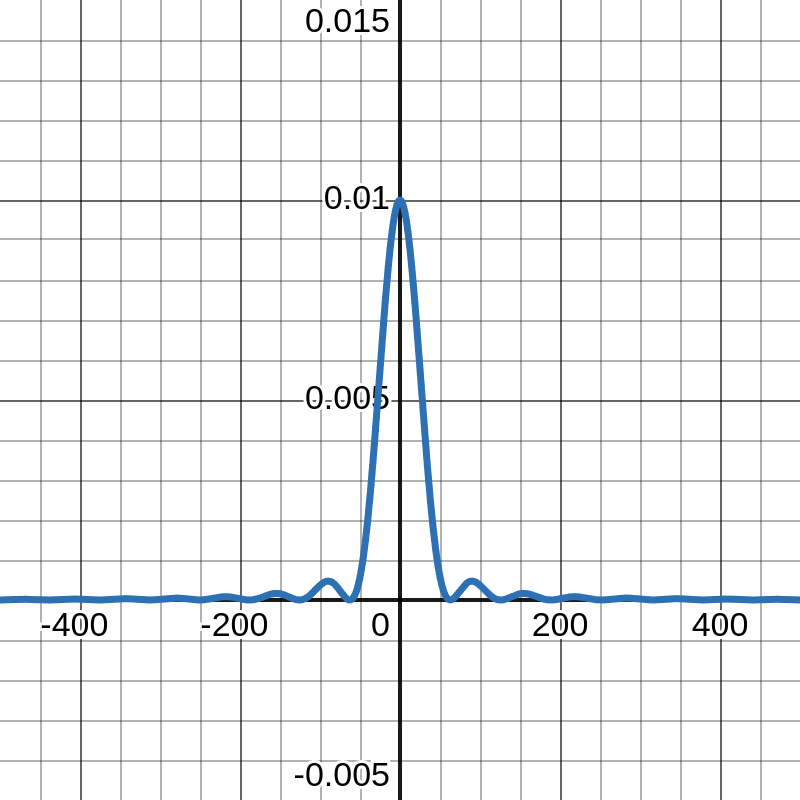
\includegraphics[width=\textwidth]{images/ej3.8}
            \caption{Densidad espectral para $x_2$}
            \label{fig:imagen2}
          \end{minipage}
        \end{figure}

        \textbf{Reflexionar:} ¿La densidad espectral es discreta o continua? ¿El gráfico admite una simetría par, impar
        o ninguna?\\

        La densidad espectral tambien es una señal de tiempo continuo, y acepta simetria par.\\

      \item Calcular la energía $E_1, E_2$ haciendo uso de la relación de Parseval.

        La relacion de Parseval indica que:

        $$E_x=\frac{1}{2\pi}\int_{-\infty}^{\infty}|\mathcal{F}\{x\}|^2$$

        Primero resolveremos la integral:
        $$
        \begin{aligned}
          \int_{-\infty}^{\infty} \Bigg[\hspace{1mm}\frac{2}{\omega} \sin\left(\frac{\omega T}{2}\right)\Bigg]^2 d\omega
          &=\int_{-\infty}^{\infty} \frac{4}{\omega^2} \sin^2\left(\frac{\omega T}{2}\right) d\omega \\[6pt]
          &= \sin^2\left(\frac{\omega T}{2}\right) \Big(-\frac{4}{\omega}\Big) - \int_{-\infty}^{\infty} 
          \Big(-\frac{4}{\omega}\Big) \frac{T}{2} \sin(\omega T)d\omega \\[6pt]
          &= \sin^2\Big(\frac{\omega T}{2}\Big)\Big(-\frac{4}{\omega}\Big) +
            2 T^2 \int \frac{\sin(\omega T)}{\omega T}d\omega \\[6pt]
          &\text{Apoyandonos en la sustitución $\omega T=x$}\\[6pt]
          &=-\sin^2\Big(\frac{\omega T}{2}\Big)\frac{4}{\omega} + 2T \int_{-\infty}^{\infty} \frac{\sin(x)}{x} dx\\[6pt]
          &=\Big[-\frac{4}{\omega} \Big(\frac{1- \cos(\omega t)}{2}\Big) + 2T Si(x)\Big]\Big|_{-\infty}^{\infty}\\[6pt]
          &=\Big[\frac{2}{\omega} (\cos(wt) - 1) + 2T Si(\omega T)\Big]\Big|_{-\infty}^{\infty}\\[6pt]
        \end{aligned}
        $$

        Desarrollando el primer termino:
        $$
        \begin{aligned}
          2\frac{\cos(\omega T)-1}{\omega} \Big|_{-\infty}^{\infty}&=2\frac{\cos(\omega T)-1}{\omega} 
          \Big|_{-\infty}^{0} + 2\frac{\cos(\omega T)-1}{\omega} \Big|_{0}^{\infty}\\[6pt]
          &= 0
        \end{aligned}
        $$

        Desarrollando el segundo termino:
        $$
        \begin{aligned}
          2T\text{Si}(\omega T)\Big|_{-\infty}^{\infty} &=
          2T\text{Si}(\omega T)\Big|_{-\infty}^{0} + 2T\text{Si}(\omega T)
          \Big|_{0}^{\infty} \\[6pt]
          &= 2T(\text{Si}(0)-\lim_{\omega \to -\infty} \text{Si}(\omega T)) +
          2T(\lim_{\omega \to \infty} \text{Si}(\omega T) - \text{Si}(0))\\[6pt]
          &=  2T\frac{\pi}{2} + 2T \frac{\pi}{2} = 2\pi T
        \end{aligned}
        $$

        De esta forma podemos afirmar que:
        $$\int_{-\infty}^{\infty} \Bigg[\hspace{1mm}\frac{2}{\omega} 
        \sin\left(\frac{\omega T}{2}\right)\Bigg]^2 d\omega= 2\pi T$$

        Siendo la energía de cada señal a travez de la relacion de persaval:
          $$E_1 = \frac{2\pi \cdot 1}{2\pi} = 1 $$
          $$E_2 = \frac{2\pi \cdot 0.1}{2\pi} = 0.1 $$

        Esto coincidide con la energía calculada en el dominio del tiempo en el punto a.\\

        Reflexionar: ¿Qué ventajas/desventajas encuentra entre el método directo para calcular la energía $E_1, E_2$ de
        las señales $x_1, x_2$ en la variable de tiempo $t$ y el método que se deriva de la relación de Parseval, en
        donde los cálculos se realizan en la variable $\omega$?

        En este caso, el metodo sobre la variable $t$ es mucho mas simple, directo y visual. En contra parte el calculo
        mediante la relación de Parseval es mucho mas tedioso, requiriendo la resolucion de una integral compleja
        y la ayuda de herramientas como la función $Si()$. Sin embargo, esto se debe a las caracteristicas de nuestra
        señal en particular, es decir que no es extensible a otros casos.

  \end{itemize}

  \item Comparar los espectros obtenidos para cada una de las señales $x_1, x_2$, evaluar y proponer las 
    características sobresalientes de ambos espectros.

    Se puede observar claramente en los graficos que los espectros obtenidos obedecen a la relación:

    $$
    \begin{aligned}
      x(t) &\leftrightarrow X(w) \\[6pt]
      x(t\alpha) &\leftrightarrow \frac{1}{|\alpha|}X\Big(\frac{w}{\alpha}\Big)
    \end{aligned}
    $$

    Esto se puede interpretar como que al ser la señal $x_1$ mas extensa en el tiempo, y por ende con cambios mas suaves
    su espectro esta concentrado en señales de frecuencia mas baja en relación al espectro de la señal $x_2$, que al ser
    mas acotada en el tiempo y por consecuencia variar mas rapidamente, su espectro presenta componentes de frecias mas
    altas.

\end{enumerate}

\chapter{}%ejercicio 4

  \textbf{Circuito Eléctrico RC:} circuito eléctrico correspondiente a un sistema de 1° orden y su ecuación
  característica:
  $$v(t) = R\cdot i(t) + \frac{1}{C} \cdot \int_{0}^{t} i(\tau) d\tau$$

  \vspace{-1cm}
  \noindent
  \begin{figure}[h]
    \centering
    \begin{minipage}[h]{0.5\textwidth}
      \centering
      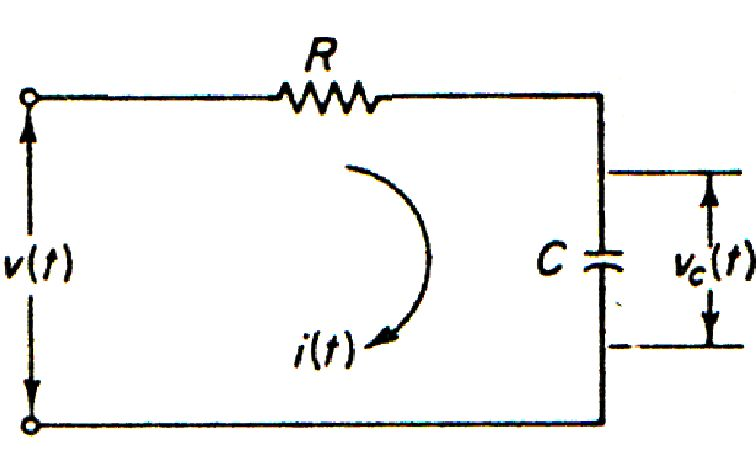
\includegraphics[width=1\textwidth]{./images/Ej4.1.jpg}
      \textit{Circuito RC}
    \end{minipage}
  \end{figure}

  \begin{enumerate}[label=\alph*)]
    \item Obtener una representación del circuito con Ecuaciones Diferenciales de primer orden y coeficientes
      constantes, y con ello, definir un Sistema en tiempo continuo con entrada $x(t) = v(t)$ y salida $y(t) = i(t)$.
      Luego, hacer un diagrama de bloques de la E.D; exponiendo los integradores que la conforma.

      El circuito RC esta descrito por la ecuacion caracteristica:
      $$v(t) = R\cdot i(t) + \frac{1}{C} \cdot \int_{0}^{t} i(\tau) d\tau$$
      Para tener una nomenclatura mas generica, sustituimos la entrada $v(t)$ con $x(t)$ y la salida $i(t)$ con $y(t)$:
      $$x(t) = R\cdot y(t) + \frac{1}{C} \cdot \int_{0}^{t} y(\tau) d\tau$$
      Teniendo en cuenta que $y(t)$ es la salida e $x(t)$ la entrada, las ecuaciones diferenciales toman la forma:
      $$\left(D^N + \sum_{i=0}^{N-1} a_i D^i\right) \cdot y(t) = \left(\sum_{i=0}^{M} b_i D^i\right) \cdot x(t)$$
      Reacomodando la ecuacion caracteristica generalizada, nos queda:
      $$
      \begin{aligned}
        y(t) + D^{-1} \left\{\frac{1}{RC} \cdot y(t) \right\} &= x(t) \cdot \frac{1}{R}\\[6pt]
        D^1\Bigl\{y(t) \Bigl\} + \frac{1}{RC} \cdot y(t) &= D^1\left\{x(t) \cdot \frac{1}{R} \right\}\\[6pt]
        \frac{dy(t)}{dt} + \frac{1}{RC} \cdot y(t) &= \frac{dx(t)}{dt} \cdot \frac{1}{R}\\[6pt]
      \end{aligned}
      $$

      Lo cual es la ecuacion diferencial de primer orden a coeficientes constantes que describe el comportamiento del
      circuito RC.

      Para el diagrama de simulacion, utilizamos la ecuacion caracteristica generalizada del sistema, solo que se
      despeja y:
      \begin{figure}[h]
        \centering
        \begin{tikzpicture}[auto, node distance=2cm, >=Stealth, thick]
          % Definición de estilos para los bloques y sumador
          \tikzstyle{block} = [draw, rectangle, minimum height=1.5em, minimum width=3em]
          \tikzstyle{sum} = [draw, circle, inner sep=1pt, minimum size=1cm, node distance=2cm]
          \tikzstyle{connector} = [fill, circle, minimum size=4pt, inner sep=0pt] % Estilo para el punto de conexión

          % Definición de nodos
          \node at (0,0) [coordinate] (input) {}; % Nodo de entrada
          \node [coordinate, right=7cm of input] (elbow1) {};
          \node [block, below=1cm of elbow1] (gain1) {$\frac{1}{R}$};
          \node [sum, below=1cm of gain1] (sum) {$+$};
          \node [block, left=2cm of sum] (integrator) {$\int$};
          \node [coordinate, left=2cm of integrator] (elbow2) {};
          \node [block, below=1cm of elbow2] (gain2) {$-\frac{1}{RC}$};
          \node [coordinate, below=1cm of gain2] (elbow3) {};
          \node [coordinate, right=4cm of sum] (output) {}; % Nodo de salida
          \node [connector, left=2cm of output] (elbow5) {};
          \node [coordinate, below=2.7cm of elbow5] (elbow4) {};

          % Conexiones entre nodos
          \draw [-] (input) -- node {$x(t)$} (elbow1);
          \draw [-] (elbow1) -- (gain1);
          \draw [->] (gain1) -- (sum);
          \draw [->] (sum) -- node {$y(t)$} (output);
          \draw [->] (integrator) -- (sum);
          \draw [->] (elbow2) -- (integrator);
          \draw [-] (gain2) -- (elbow2);
          \draw [->] (elbow3) -- (gain2);
          \draw [-] (elbow4) -- (elbow3);
          \draw [-] (elbow5) -- (elbow4);
        \end{tikzpicture}
        $$y_t = \frac{x_t}{R} + D^{-1}\left\{-\frac{y_t}{RC}\right\}$$
      \end{figure}

    \item Teniendo en cuenta el siguiente resultado matemático, obtener una descripción explicita
      de la respuesta $y(t)$ del sistema obtenido en el inciso anterior:
      \begin{itemize}
        \item Sean $\alpha, \beta_0, \beta_1 \in \mathbb{R}$ constantes; $y(t), x(t)$ funciones con variable de tiempo continuo,
          las cuales verifican la ecuación diferencial de primer orden con coeficientes constantes:

          $$y_t'+\alpha y_t = \beta_1 x_t' + \beta_0 x_t$$

          Entonces, una Solución General explicita de la Ecuación Diferencial es

          $$y_t = \beta_1 x_t + (y_0 - \beta_1 x_0) e^{-\alpha t} + (\beta_0 - \alpha \beta_1) \int_{0}^{t} x(\tau)
          e^{-\alpha(t - \tau)} d\tau$$

          donde $y_0 = y(0), x_0 = x(0)$ son Condiciones Iniciales arbitrarias
        \end{itemize}

        Identificando los coeficientes $\alpha, \beta_0, \beta_1$, tenemos lo siguiente:
        $$\alpha = \frac{1}{RC}; \hspace{1cm}\beta_0 = 0; \hspace{1cm}\beta_1 = \frac{1}{R}$$
        Por lo tanto, la solucion general explicita para el $S_1\{x_t\}$ es:
        $$y_t = S_1\{x_t\} = x_t \cdot \frac{1}{R} + \left(y_o - \frac{x_0}{R}\right) \cdot e^{\frac{-t}{RC}} -
        \frac{1}{R^2C} \int_{0}^{t} x_\tau \cdot e^{\frac{-(t-\tau)}{RC}} d\tau$$


    \item Usando la descripción explicita de la salida del Sistema $y_t = S_1{x_t}$ (CI arbitrarias) del inciso
      anterior, calcular la respuesta a cada una de las siguientes señales:
      $$x_0(t) = 0, \hspace{0.5cm}x_1(t) = \mu_t, \hspace{0.5cm}x_2(t) = \mu(t - t_0), \hspace{0.5cm}x_3(t) =
      \mu_t - \mu(t - t_0), \hspace{0.5cm}x_4(t) = t$$

      \textbf{Reflexionar:} ¿La señal $y_0$ es completamente nula? ¿Las señales $y_3, y' = y_1 - y_2$ (iguales o
      distintas)? ¿es suficiente para garantizar la Linealidad del sistema? ¿Las señales $y_1, y_2$ son iguales? ¿es
      suficiente para garantizar la Inv. Tiempo del sistema?.

      Solucion para $x_t = x_0 = 0$:
      \begin{align*}
        y_0(t) &= 0 \cdot \frac{1}{R} + \left(y_0 - \frac{x_0}{R}\right) \cdot
          e^{\frac{-t}{RC}} - \frac{1}{R^2C} \int_{0}^{t} 0 \cdot e^{\frac{-(t-\tau)}{RC}} d\tau\\[6pt]
        y_0(t) &= \left(y_0 - \frac{x_0}{R}\right) \cdot e^{\frac{-t}{RC}}
      \end{align*}
      Como se puede ver, la señal $y_0$ no es completamente nula. Esta presenta una exponencial decreciente para
      $t > 0$. Seria nula en caso de que las C.I. sean nulas, o que se cumpla que $y_0 = x_0/R$.\\

      Solucion para $x_t = x_1 = \mu_t$:
      \begin{align*}
        y_1(t) &= \mu_t \cdot \frac{1}{R} + \left(y_0 - \frac{x_0}{R}\right) \cdot
          e^{\frac{-t}{RC}} - \frac{1}{R^2C} \int_{0}^{t} \mu_t \cdot e^{\frac{-(t-\tau)}{RC}} d\tau\\[6pt]
        y_1(t) &= \mu_t \cdot \frac{1}{R} + \left(y_0 - \frac{x_0}{R}\right) \cdot e^{\frac{-t}{RC}} -
          \frac{1}{R^2C} \int_{0}^{t} e^v \cdot RCdv\\[6pt]
        y_1(t) &= \mu_t \cdot \frac{1}{R} + \left(y_0 - \frac{x_0}{R}\right) \cdot e^{\frac{-t}{RC}} -
          \frac{1}{R} \left[e^{\frac{-(t-\tau)}{RC}}\right]\Big|_{0}^{t}\\[6pt]
        y_1(t) &= \mu_t \cdot \frac{1}{R} + \left(y_0 - \frac{x_0}{R}\right) \cdot e^{\frac{-t}{RC}} - \frac{1}{R}
          \left[1 - e^{\frac{-t}{RC}}\right]
      \end{align*}
      Solucion para $x_t = x_2 = \mu_{t-1}$:
      \begin{align*}
        y_2(t) &= \mu_{t-1} \cdot \frac{1}{R} + \left(y_0 - \frac{x_0}{R}\right) \cdot
          e^{\frac{-t}{RC}} - \frac{1}{R^2C} \int_{0}^{t} \mu_{t-1} \cdot e^{\frac{-(t-\tau)}{RC}} d\tau\\[6pt]
        y_2(t) &= \mu_{t-1} \cdot \frac{1}{R} + \left(y_0 - \frac{x_0}{R}\right) \cdot e^{\frac{-t}{RC}} -
          \frac{1}{R^2C} \int_{1}^{t} e^v \cdot RCdv\\[6pt]
        y_2(t) &= \mu_{t-1} \cdot \frac{1}{R} + \left(y_0 - \frac{x_0}{R}\right) \cdot e^{\frac{-t}{RC}} -
          \frac{1}{R} \left[e^{\frac{-(t-\tau)}{RC}}\right]\Big|_{1}^{t}\\[6pt]
        y_2(t) &= \mu_{t-1} \cdot \frac{1}{R} + \left(y_0 - \frac{x_0}{R}\right) \cdot e^{\frac{-t}{RC}} -
          \frac{1}{R} \left[1 - e^{\frac{1-t}{RC}}\right]
      \end{align*}
      Solucion para $x_t = x_3 = \mu_t - \mu_{t-1}$:
      \begin{align*}
        y_3(t) &= (\mu_t - \mu_{t-1}) \cdot \frac{1}{R} + \left(y_0 - \frac{x_0}{R}\right) \cdot e^{\frac{-t}{RC}} -
          \frac{1}{R^2C} \int_{0}^{t} (\mu_t - \mu_{t-1}) \cdot e^{\frac{-(t-\tau)}{RC}} d\tau\\[6pt]
        y_3(t) &= (\mu_t - \mu_{t-1}) \cdot \frac{1}{R} + \left(y_0 - \frac{x_0}{R}\right) \cdot e^{\frac{-t}{RC}} -
          \frac{1}{R^2C} \left[\int_{0}^{t} \mu_t \cdot e^{\frac{-(t-\tau)}{RC}} d\tau -
          \int_{0}^{t} \mu_{t-1} \cdot e^{\frac{-(t-\tau)}{RC}} d\tau \right]\\[6pt]
        y_3(t) &= (\mu_t - \mu_{t-1}) \cdot \frac{1}{R} + \left(y_0 - \frac{x_0}{R}\right) \cdot e^{\frac{-t}{RC}} -
        \frac{1}{R^2C} \left[\int_{0}^{t} e^{\frac{-(t-\tau)}{RC}} d\tau -
          \int_{1}^{t} e^{\frac{-(t-\tau)}{RC}} d\tau \right]\\[6pt]
        y_3(t) &= (\mu_t - \mu_{t-1}) \cdot \frac{1}{R} + \left(y_0 - \frac{x_0}{R}\right) \cdot e^{\frac{-t}{RC}} -
          \frac{1}{R^2C} RC\left[\int_{0}^{t} e^v dv - \int_{1}^{t} e^v dv \right]\\[6pt]
        y_3(t) &= (\mu_t - \mu_{t-1}) \cdot \frac{1}{R} + \left(y_0 - \frac{x_0}{R}\right) \cdot e^{\frac{-t}{RC}} -
          \frac{1}{R}\left[e^{\frac{-(t-\tau)}{RC}} \Big|_{0}^{t} -
          e^{\frac{-(t-\tau)}{RC}} \Big|_{1}^{t} \right]\\[6pt]
        y_3(t) &= (\mu_t - \mu_{t-1}) \cdot \frac{1}{R} + \left(y_0 - \frac{x_0}{R}\right) \cdot e^{\frac{-t}{RC}} -
          \frac{1}{R} \left[e^{\frac{1-t}{RC}} - e^{\frac{-t}{RC}}\right]
      \end{align*}
      Solucion para $y' = y_1 - y_2$:
      \begin{align*}
        y' &= \mu_t \cdot \frac{1}{R} + \left(y_0 - \frac{x_0}{R}\right) \cdot e^{\frac{-t}{RC}} - \frac{1}{R}
          \left[1 - e^{\frac{-t}{RC}}\right] - \left(\mu_{t-1} \cdot \frac{1}{R} + \left(y_0 -
          \frac{x_0}{R}\right) \cdot e^{\frac{-t}{RC}} - \frac{1}{R} \left[1 - e^{\frac{1-t}{RC}}\right]\right)\\[6pt]
        y' &= (\mu_t - \mu_{t-1}) \cdot \frac{1}{R} - \frac{1}{R} \left[e^{\frac{1-t}{RC}} - e^{\frac{-t}{RC}}\right]
      \end{align*}
      Como se puede ver, $y' \neq y_3$. Esto significa que el sistema $S_1\left\{x_t\right\}$ no es lineal. Se puede
      ver que si las condiciones lineales son nulas, o si $y_0 = x_0/R$, la igualdad se cumple, y el sistema es lineal.
      Por otro lado, las ecuaciones $y_1 \neq y_2$, ademas, con ellas no se puede demostrar la invarianza en el tiempo,
      debido a que por un lado, se debe desplazar la señal de entrada, y por otro lado, se debe desplazar la señal de
      salida, para verificar que el sistema es invariante en el tiempo.\\

      Solucion para $x_t = x_4 = t$:
      \begin{align*}
        y_4(t) &= t \cdot \frac{1}{R} + \left(y_0 - \frac{x_0}{R}\right) \cdot e^{\frac{-t}{RC}} -
          \frac{1}{R^2C} \int_{0}^{t} \tau \cdot e^{\frac{-(t-\tau)}{RC}} d\tau\\[6pt]
        y_4(t) &= t \cdot \frac{1}{R} + \left(y_0 - \frac{x_0}{R}\right) \cdot e^{\frac{-t}{RC}} -
          \frac{1}{R^2C} \left[\tau \cdot RC e^{\frac{-(t-\tau)}{RC}} - RC\int e^{\frac{-(t-\tau)}{RC}} d\tau\right]
          \Big|_{0}^{t}\\[6pt]
        y_4(t) &= t \cdot \frac{1}{R} + \left(y_0 - \frac{x_0}{R}\right) \cdot e^{\frac{-t}{RC}} -
          \frac{1}{R} \left[\tau \cdot e^{\frac{-(t-\tau)}{RC}} - RC\int e^v dv\right] \Big|_{0}^{t}\\[6pt]
        y_4(t) &= t \cdot \frac{1}{R} + \left(y_0 - \frac{x_0}{R}\right) \cdot e^{\frac{-t}{RC}} -
          \frac{1}{R} \left[\tau \cdot e^{\frac{-(t-\tau)}{RC}} - RC e^{\frac{-(t-\tau)}{RC}} \right]
          \Big|_{0}^{t}\\[6pt]
        y_4(t) &= t \cdot \frac{1}{R} + \left(y_0 - \frac{x_0}{R}\right) \cdot e^{\frac{-t}{RC}} -
          \frac{1}{R} \left[e^{\frac{-(t-\tau)}{RC}} (\tau - RC)\right] \Big|_{0}^{t}\\[6pt]
        y_4(t) &= t \cdot \frac{1}{R} + \left(y_0 - \frac{x_0}{R}\right) \cdot e^{\frac{-t}{RC}} -
          \frac{1}{R} \left[t - RC + RC e^{\frac{-t}{RC}}\right]\\[6pt]
      \end{align*}

    \item Usando la descripción explicita de la salida del Sistema $y_t = S_1{x_t}$ (CI arbitrarias), demostrar si el
      Sistema $S1$ es (o no): Lineal, Homogéneo e Invariante en el Tiempo.

    \item Demostrar que el sistema anterior en reposo gana propiedades, esto es, definir $y_t = S_2{x_t}$ con C.I. 
      nulas $y_0 = x_0 = 0$, y clasificar el sistema S2 (Aditivo, Homogéneo, Inv. Tiempo).

    \item Refinar aun más el sistemas, exijamos C.I nulas y respuesta causal (se elimine el pasado), esto es, definir 
      $y_t = S_3{x_t} = S_2{x_t} \mu_t$. Demostrar que el sistema S3 es LIT (Lineal e Inv. Tiempo). Sintetizar sus 
      respuestas es una tabla de doble entrada:

      \begin{table}[h!]
        \centering
        \begin{tabular}{|c|c|c|c|}
          \hline
          \textbf{Entrada $x_t$} & \textbf{Salida $y_t = S_3{x_t}$} & \textbf{Salida $y_t = x_t * h_t$} & \textbf{Comparar}\\
          \hline
          $\delta_t$ & $h_t = ??$ & &\\
          \hline
          $\mu_t$ & & &\\
          \hline
          $\mu_{t-1}$ & & &\\
          \hline
          $\mu_t - \mu_{t-1}$ & & &\\
          \hline
          $t$ & & &\\
          \hline
          $t\mu_{t}$ & & &\\
          \hline
          $e^{2t}$ & & &\\
          \hline
          $e^{2t}\mu_{-t}$ & & &\\
          \hline

        \end{tabular}
      \end{table}
      \textbf{Reflexionar:} En general, ¿cualquier sistema $S$ admite una descripción del tipo $S{x} = y = x * h$?
      ¿Cuales son los requerimientos para que esto suceda? ¿El dominio de señales de entrada del sistema linealizado
      $S_3{x}$, es igual al dominio del sistema $x * h$?


  \end{enumerate}

  \textbf{Circuito Eléctrico RLC:} circuito eléctrico correspondiente a un sistema de 2° orden y su ecuación caracteristica: $v(t) = Ri_{(t)} + L \frac{d}{dt} i_{(t)} + \frac{1}{C} \int_{0}^{t} i_{(\tau)} d\tau$

  \begin{enumerate}[label=\alph*)]
  \item Obtener una representación del circuito con Ecuaciones Diferenciales de segundo orden y coeficientes constantes, y con ello, definir un Sistema en tiempo continuo con entrada $x_{(t)} = v_{(t)}$ y salida $y_{(t)} = i_{(t)}$. Luego, hacer un diagrama de bloques de la E.D; exponiendo los integradores que la conforma.

  \item Sea $y_t = S\{x_t\}$ el sistema obtenido de las soluciones al sistema de Ecuaciones Diferenciales del inciso anterior. Teniendo en cuenta el siguientes resultado matemático, obtener una descripción explicita de la respuesta transformada $Y_{(s)} = L\{y_t\} = L\{S\{x_t\}\}$:
  \begin{itemize}
    \item Sean $\alpha_1, \alpha_0, \beta_2, \beta_1, \beta_0 \in \mathbb{R}$ constantes; $y_{(t)}, x_{(t)}$ funciones con variable de tiempo continuo, las cuales verifican la ecuacion diferencial de segundo orden con coeficientes constantes:
    $$y_t^{''} + \alpha_1 y_t^{'} + \alpha_0 y_t = \beta_2 x_t^{''} + \beta_1 x_t^{'} + \beta_0 x_t$$
    Entonces, una Solucion General explicita de la Ecuacion Diferencial Transformada es:
    $$Y_{(s)} = \frac{\beta_2 s^2 + \beta_1 s + \beta_0}{s^2 + \alpha_1 s + \alpha_0}X_{(s)} + \frac{(y_0 - \beta_2 x_0)s + (\alpha_1 y_0 - \beta_1 x_0 + y_0^{'} - \beta_2 x_0^{'})}{s^2 + \alpha_1 s + \alpha_0}$$
    donde $Y_{(s)} = L\{y_t\}$, $X_{(s)} = L\{x_t\}$, con $s = \sigma + j \omega$ (variable compleja). Condiciones Iniciales arbitrarias; $y_0 = y(0), y_0^{'} = y^{'}(0), x_0 = x(0), x_0^{'} = x^{'}(0)$.
    \item Usando las propiedades de la transformada de Laplace, demostrar la igualdad propuesta para la funcion $Y_{(s)}$.
  \end{itemize}

  \item Restringir el sistema anterior a CI nulas y obtener la formula de la respuesta transformada $Y_{(s)} = L\{y\}$. Luego, calcular la Función de transferencia $H_{(s)} = L\{h_t\}$ donde $h_t$ es la respuesta al impulso del sistema linealizado. Luego, graficar en el plano complejo los polos y ceros de dicha función.

  \item Trabajar con el sistema linealizado del inciso anterior, y calcular la transformada $Y_1(s) = L\{S\{3\delta_{(t-2)}\}\}$, y similarmente $Y_2(s) = L\{S\{\mu_{(t+2)}\}\}$. Luego, implementar la técnica de anti-transformada para obtener las señales de respuesta en la variable de tiempo $y_1 = S\{3\delta_{(t-2)}\}$, $y_2 = S\{\mu_{(t+2)}\}$, respectivamente.\\
  \textbf{Reflexionar}: ¿En que variable están definidas las funciones $Y_1$, $Y_2$? ¿Que tipo de variable es $s$ y que diferencia tiene con la variable $t$? ¿Que diferencias se observan entres las funciones $Y_1$, $Y_2$ y sus señales $y_1$, $y_2$?

  \item Graficar en diagrama de bloques del sistema en el dominios de la variable compleja.  Determinar el coeficiente de amortiguamiento $\xi$ y la frecuencia natural $\omega_n$ del sistema linealizado.\\
  \textbf{Reflexionar}: ¿Que diferencias se observan entre el diagrama de bloques del inciso (a) y el diagrama de bloques del inciso (e)? ¿Las variables $s$ y $t$ están presentes de alguna forma en los diagramas mencionados? ¿Tiene algún significado subrayar que el diagrama esta en el dominio del tiempo o en el dominio complejo?

  \end{enumerate}
\end{document}
